\chapter{Introduction} \label{introduction}

An organism's capabilities are encoded by the sequence of nucleotides found within its DNA \cite{crick1970central}. DNA sequencing \footnote{Genome sequencing involves taking multiple copies of an organism's genome, fragmenting them randomly, and placing them into a sequencing machine \cite{shendure2017dna}. This machine reads the sequence of nucleotides in each fragment \cite{shendure2017dna}. These potentially overlapping fragments are sequenced in parallel for higher throughput. After sequencing, the order of nucleotides of these fragments is the used, \textit{in silico}, to assemble a readout of the organism's entire genome sequence \cite{wajid2012review}. The assembly process involves stitching together overlapping fragments with highly similar head and tail sequences, which is analogous to putting together pieces of a puzzle \cite{wajid2012review}.} allows us to read these sequences and, through software, learn more about an organism's inherent capabilities without having to study it \textit{in vivo} or \textit{in vitro} \cite{de2012bioinformatic}. In an environmental microbiology context, such sequenced genomes are used to learn more about microorganisms' metabolic capabilities and possibly shed light on their ecological role \cite{de2012bioinformatic}. In an applied context, predictions of such metabolic capabilities are also useful. Certain microbes are more suitable for specific bioprocesses \footnote{A bioprocess is a process carried out by living cells or their components. They are used across a variety of industrial sectors including energy \cite{deublein2011biogas}, mining \cite{dew1997biox}, manufacturing \cite{thodey2014microbial}, and environmental remediation \cite{alexander1999biodegradation}.} and this suitability is based on these organism's metabolisms. The metabolisms involved influence the process's conditions and overall efficiently \cite{doran1995bioprocess,liu2016bioprocess}. In both applied and environmental contexts, genomically derived genome-scale metabolic reconstruction models can be used to simulate nutrient flow through and between organisms \cite{magnusdottir2017generation, arkin2018kbase, faria2018improving}. In a genetic engineering context, genomically derived information can be used to select what traits to remove from organisms or move between them \cite{strohl2001biochemical}. These traits can even be metabolic \cite{sanchez2005novel}.

Advances in DNA sequencing technology over the past decade have revolutionized our ability to acquire bacterial and archaeal genomes. For example, with newer sequencing technologies such as Oxford Nanopore \cite{jain2016oxford}, a bacterial genome can be acquired in a matter of hours \cite{Lu2016,Cao2017}. Researchers have now moved on to extracting the genomes of unculturable microorganisms from environmental samples using culture-free techniques such a metagenomic \cite{quince2017shotgun} and single-cell \cite{gawad2016single} sequencing. Over the past few years, the tree of life has been significantly expanded by the Metagenome Assembled Genomes (MAGs) \footnote{Shotgun metagenomics involves sequencing the genomes of a mixture of organisms in parallel \cite{quince2017shotgun}. The resulting sequenced fragments are not labelled as to what organism they came from. In software, genome assembly and an additional step called genome binning are used to generate multiple genomes out of the pool of sequenced fragments produced by the sequencer \cite{quince2017shotgun, sangwan2016recovering}. If they are of high completeness and low in contamination, these separated genomes are called Metagenome Assembled Genomes (MAGs)  \cite{sangwan2016recovering}. \label{metagenomics-footnote}} of these unculturable organisms \cite{Hug2016,Parks2017}. With microbiologists' ability to gather new genomes rectified, the problem now shifts to interpreting this new wealth of genomic data.

Due to their vast size and information density, the interpretation of genomes is often assisted by software. The tool developed as part of the thesis work, Micromeda, is such a piece of software and allows users to generate data visualizations that help them identify patterns in the presence and absence of biochemical pathways across organisms. Pygenprop, a library built to assist in the development of Micromeda, will enable users to perform such comparisons programmatically. A key feature of both Micromeda and Pygenprop is their ability to not only compare the predicted metabolic features of organisms, in terms of biochemical pathways present but also allow users to access the underlying protein sequences that support these predictions. Details about the information presented by Micromeda and its expected use cases are presented within the sections below. The following chapters will discuss the database Micromeda uses, Pygenprop and Micromeda's implementation.

\section{Enzymes and Biochemical Pathways} \label{enzymes-and-pathways} 

For many systems, both environmental and industrial processes can be carried out biochemically. From a biological context, such processes are carried out via a series of chemical reactions catalyzed by biological enzymes. Enzymes act as biological catalysts that accelerate chemical reactions via the lowering their required activation energy \cite{segel1975enzyme}. The majority of enzymes are made from protein \cite{kruger1982self}. According to the central dogma of molecular biology, all proteins, whether structural or enzymatic, within cells are encoded for by genes that are a subset of an organism's DNA-based genome \cite{crick1970central}. Within prokaryotic \footnote{Bacteria and Archaea from two distinct branches of the tree of life. The cells of these prokaryotic organisms generally\cite{nevo2007thylakoid,cameron2013biogenesis,bazylinski2004magnetosome,van2008combined,adams2000heterocyst,o2000biofilm} lack membrane-bound cellular compartments (organelles) and are unicellular. The rest of the tree of life is made up of eukaryotes that have organelles and can be multicellular \cite{baldauf2003deep}. Plants, animals and fungi are eukaryotes. \label{types-of-cells}} organisms such as Archaea and Bacteria, most often one gene maps to one protein, or protein subunit, produced. In Eukaryotes (see Footnote \ref{types-of-cells}), one gene may map to multiple proteins \cite{black2003mechanisms}. When a cell requires an enzyme, the DNA gene providing a blueprint for it is transcribed to RNA transcripts \cite{crick1970central}. These transcripts later provide instructions to a ribosome on how to join a series of ammo acid residues together into a specific polypeptide biopolymer \cite{crick1970central}. This biopolymer then spontaneously folds, based on chemical properties of its amino acid residues, into a unique three-dimensional shape that forms an enzymatic protein \cite{fersht1992folding}. The order of the residues in the polypeptide that forms a protein, which is encoded for by its DNA gene, is crucial to an enzyme's folded shape and activity towards different chemical reactions. This order is called a sequence and is also crucial for determining what chemical compounds, called substrates, are most likely to be used as inputs into a reaction catalyzed by an enzyme \cite{fersht1992folding,fersht1999structure}. Mutations in the gene's sequence can cause changes in substrate specificity (i.e., what compounds are most likely for an enzyme to use as inputs into a reaction). The genes that encode for enzymes are often under selective pressure (i.e., organisms with more efficient enzymes may produce more offspring) and thus evolve \cite{zhang2003evolution,whelan2001general}. Often genes are duplicated, and duplicates are free to evolve to tackle new substrates \cite{zhang2003evolution}. All genes are derived from the duplication and mutation of other genes, and thus all enzymes are related to all other enzymes \cite{zhang2003evolution,whelan2001general}. Thus, enzymes that facilitate similar chemical reactions often \cite{galperin1998analogous} have similar sequences of amino acid residues, structures and genes that encode them \cite{zhang2003evolution}.


A biochemical pathway represents a series of chemical reactions, that when chained together, are beneficial to a cell \cite{michal2012biochemical}. Examples of such reactions are the breaking down of a nutrient macromolecule into pieces that cells can use or the build-up of components of cellular structure \cite{wagner2012metabolic}. Each reaction step in a pathway is often \cite{keller2015widespread,tawfik2010enzyme} catalyzed by a specific enzyme whose amino acid sequence, and thus structure and activity, is optimized for the reaction \cite{michal2012biochemical,zhang2003evolution,fersht1999structure}. Thus, there is a mapping between specific enzymes (and the genes encoding them) and chemical reaction steps in biochemical pathways \cite{thiele2010protocol}. As a result, by reading the genome, researchers can predict what biochemical pathways an organism may possess \cite{abubucker2012metabolic,thiele2010protocol}. Genes encoding for enzymes that all assist in the same biochemical pathway are often co-located spatially on a host's genome \cite{lawrence1999selfish,de2010genomic}. Sometimes these genes are transcribed together before translation into individual proteins \cite{blumenthal1998gene,danchin1980coordinate}. Due to the evolution of genes and enzymes over time, biochemical pathways can also change over time \cite{hochachka2002biochemical,raymond2006effect}. New enzymes or derivatives of existing enzymes can replace those enzymes that catalyzed pathway steps in the past \cite{jensen1976enzyme}. This swapping also follows evolutionary patterns \cite{morowitz1999theory, raymond2006effect,wagner2012metabolic}. Organisms from different environments may have different enzymes that catalyse pathway reactions in a different way \cite{raymond2006effect}. Often chemical compounds produced halfway through a pathway can be used as inputs for an entirely different pathway \cite{wagner2012metabolic,stelling2002metabolic}. Also, the output from one pathway (e.g. the monomers from the break down of a macro-nutrient) may be the input for a second biochemical pathway that builds cellular structures \cite{wagner2012metabolic,stelling2002metabolic}. Thus, all pathways in a cell are somehow connected and form a network of reactions \cite{wagner2012metabolic,stelling2002metabolic}. This network forms the cell's metabolism and is called its metabolic network \cite{wagner2012metabolic}.


\section{Pathway Databases}

For many decades scientists have been designing and executing studies to figure out what individual enzymes do and what substrates they can catalyze. They have also found what genes encode for these enzymes. The results of such studies are stored in pathway databases. Specifically, what genes encode for what enzymes, what enzymes catalyze what reactions, and what reactions belong to what biochemical pathways. These databases also map how pathways are connected within cells' metabolic networks. Examples of such databases include KEGG \cite{kanehisa2000kegg}, MetaCyc \cite{karp2002metacyc}, Genome Properties \cite{richardson2018genome}, SEED subsystems \cite{overbeek2005subsystems}, Reactome \cite{croft2013reactome}, and many others. Such databases are often optimized to contain data about a specific organism (e.g. humans \cite{croft2013reactome}), clade on the tree of life (e.g. prokaryotes \cite{richardson2018genome}) or area of metabolism (e.g. small molecule production \cite{Jewison2014}).

\section{The State of Pathway Analysis}

As the breadth of the information within pathway databases increases, it is increasingly being used for the automation of pathway analysis. Researchers are automating their workflows by developing software tools that help them predict the presence of pathways in novel organisms or build models that predict the flux of nutrients through cells. Such tools help them make rapid insights into the capabilities and roles of organisms in a variety of environments. Often this software is released in the form of a toolchain (i.e., a pipeline) where a separate bioinformatics software application performs each step. Such pipelines take an organism's DNA genome sequence, perform \textit{in-silico} transcription and translation (Fig. \ref{fig:pathway-analysis-steps}), identify enzymes, and figures out what pathways they belong to via information contained within pathway databases (Fig. \ref{fig:pathway-analysis-overview}). These tools perform some or all of the following key steps.

\begin{enumerate}
\item Prediction of what genes are present in an organism's genome.
\item Translation of these genes' sequences to protein for reduced redundancy (Fig. \ref{fig:pathway-analysis-steps}). \footnote{There are four types of nucleotide monomers in the DNA biopolymer. Each is assigned a letter A, T, C or G. For protein-coding genes, three-letter codes (e.g. ATC, or CCG) in the DNA sequence, called codons, map to specific amino acids added to the translated protein sequence. Various types of three-letter codes can cause the addition of a single type of amino acid. Storing protein sequences instead of DNA sequences reduces redundancy in two ways. Firstly, by reducing the length of the information to be stored by one third due to a three to one letter mapping between DNA and protein sequences. Secondly, by replacing multiple sets of three DNA letters with a single amino acid letter due to codon to amino acid mappings. An added benefit is that translation of DNA sequences to protein is that it masks mutations in the DNA sequence that do not change a protein's sequence and thus its enzymatic function.} 
\item Taking known enzymatic protein sequences from pathway databases and using them to search the above-predicted proteins to find those with high sequence similarity. Predicted proteins with high sequence similarity to known enzymes are likely to carry out the same enzymatic function (see Section \ref{enzymes-and-pathways}). This process is called protein annotation (Fig. \ref{fig:pathway-analysis-steps}).
\item Using these newly found enzymes to figure out what chemical reactions could be carried out by an organism.
\item Chaining these reactions together to figure out what biochemical pathways are likely to be possessed by the organism (Fig. \ref{fig:pathway-analysis-steps}). This process is called pathway annotation.
\item Presentation of information about the pathways present and enzymes found in a way that is comprehensible by users.
\end{enumerate}

\begin{figure}[!ht]
  \centering
	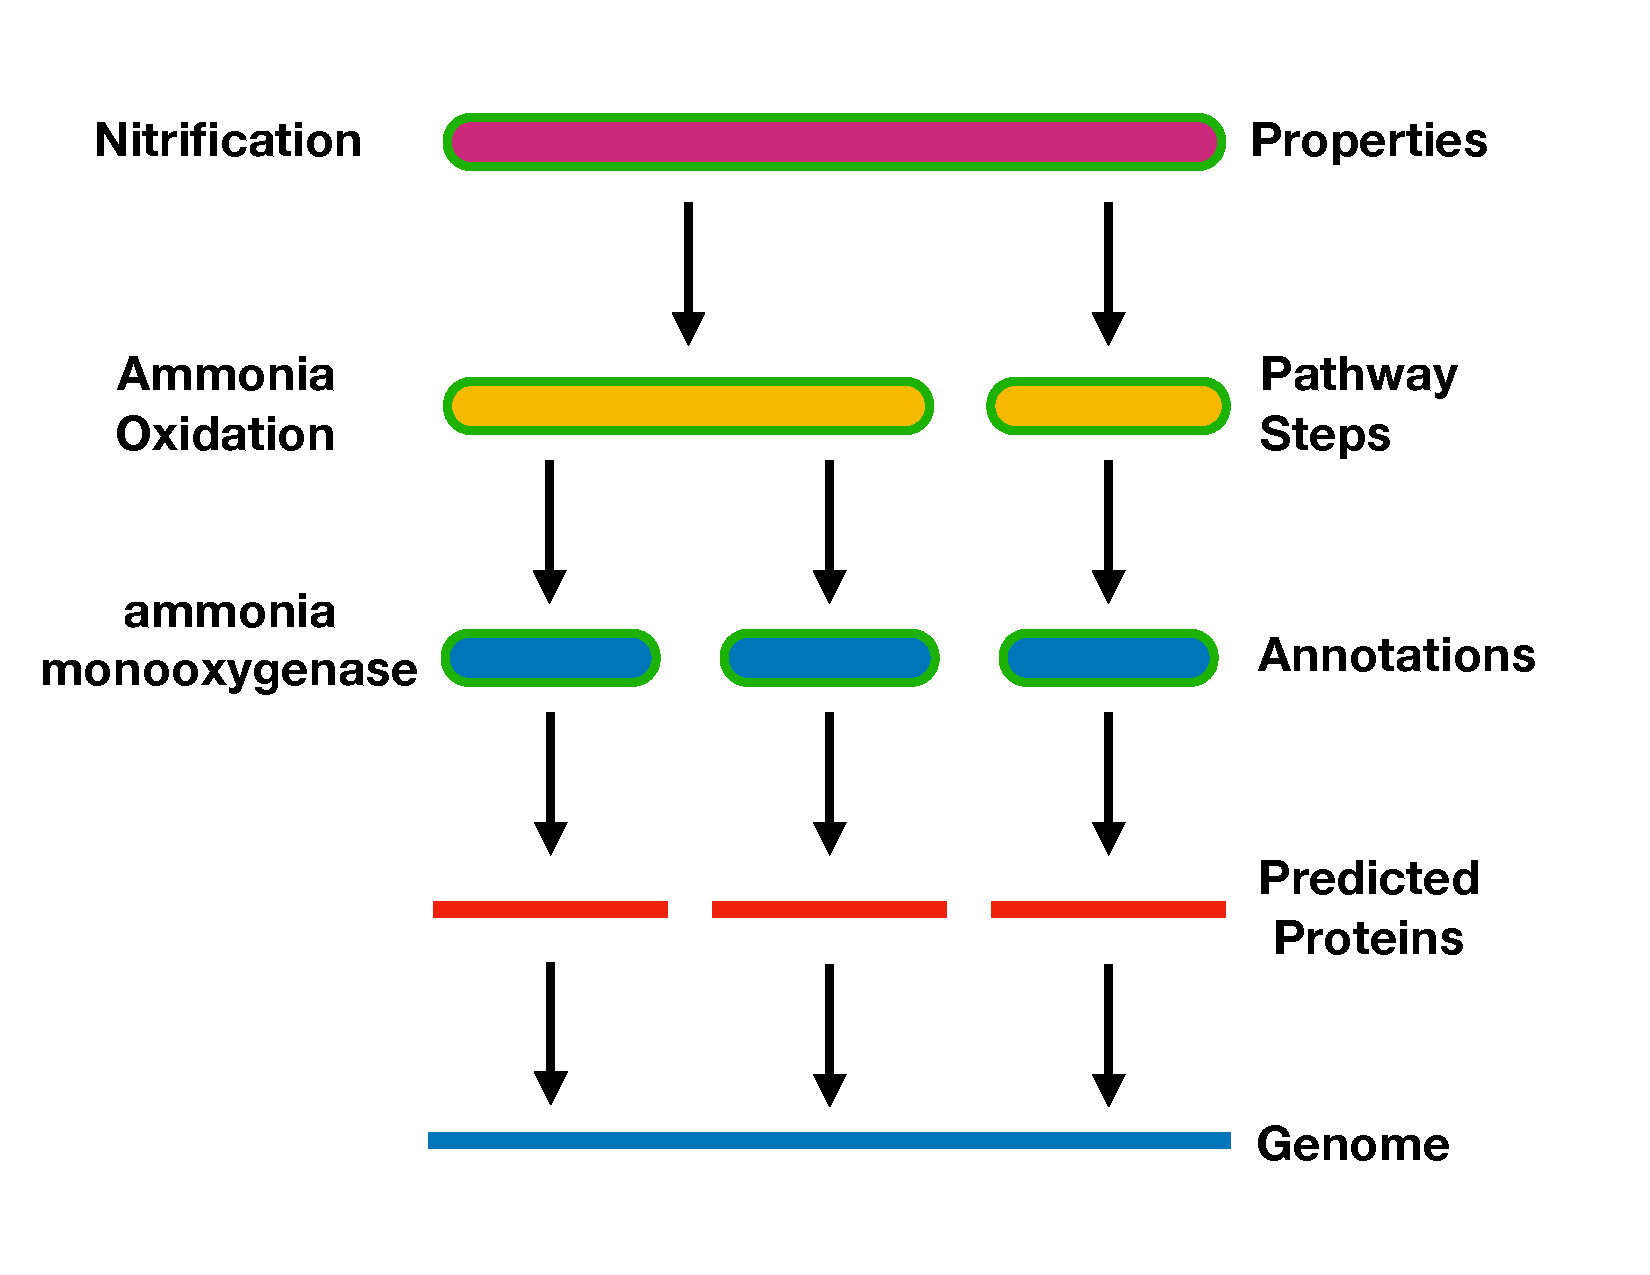
\includegraphics[width=0.8\textwidth]{media/pathway_analysis_steps.pdf}
	 \caption{Several steps are required to go from an organism's genome sequence to a prediction of its metabolic capabilities.}
	 \label{fig:pathway-analysis-steps}
\end{figure}

\begin{figure}[!ht]
  \centering
	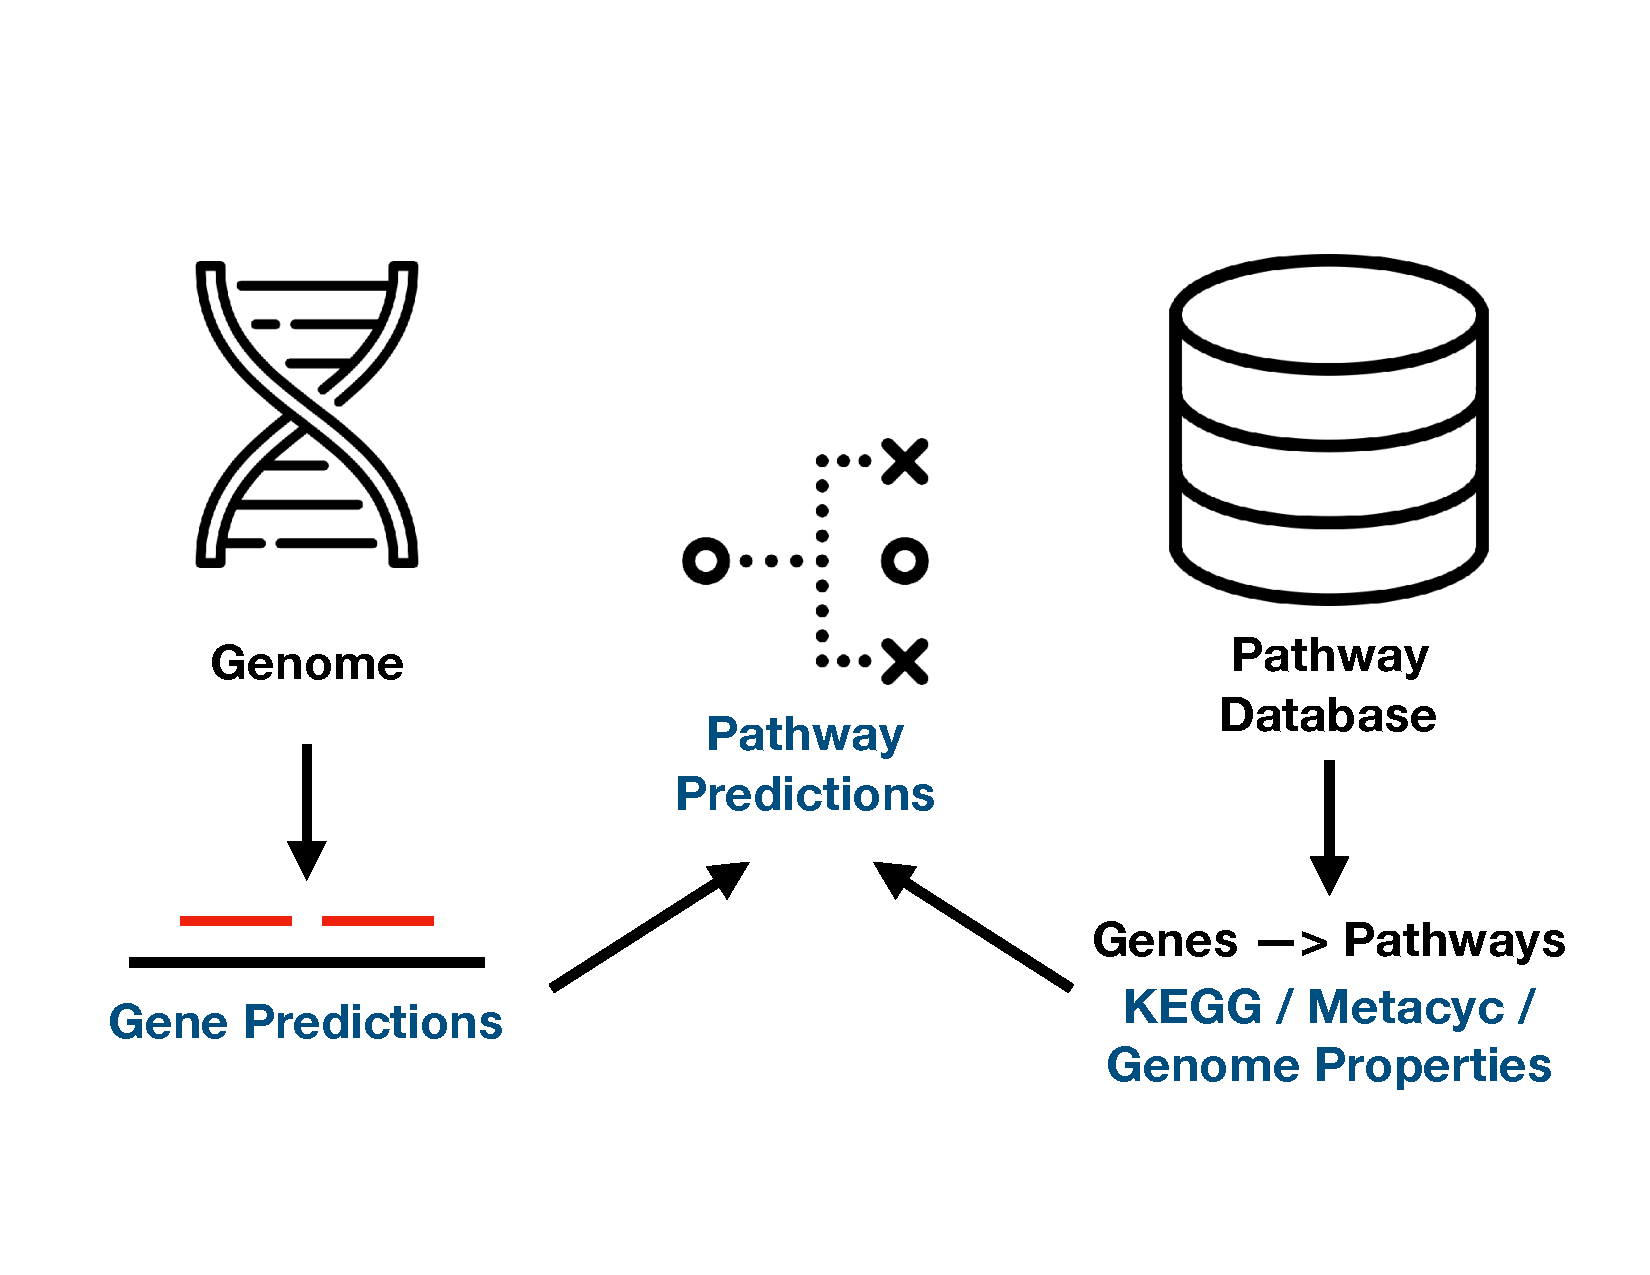
\includegraphics[width=0.8\textwidth]{media/pathway_bioinformatics.pdf}
	 \caption{Predicting the biochemical pathways that an organism may possess involves combining a predictions of what genes an organisms possesses with information about what genes are required by what pathways.}
	 \label{fig:pathway-analysis-overview}
\end{figure}

Some pipelines only work with pathway data from a specific database. For example, Pathway Tools \cite{karp2002pathway} can only present information about pathways found within the MetaCyc \cite{karp2002metacyc} database. Often pipelines are optimized for generating data from the genomes of a specific clade on the tree of life. For example, Prokka \cite{seemann2014prokka}, a pipeline that predicts genes and annotates protein sequences, is only designed to work with the genomes of prokaryotic microbes. Prokka only carries out the first few steps of the above list \cite{seemann2014prokka}. Some tools can perform all of the above steps. For example, the metagenomics pipeline Automatic Tool for Local Assembly Structures (ATLAS) \cite{white2017atlas,kieser2019atlas} can perform, in addition to generating genomes from raw sequencing reads, pathway annotation. ATLAS uses Prokka internally for some of its steps \cite{white2017atlas,kieser2019atlas}. Users can deploy such bioinformatics pipelines in two ways. They can either be installed on to a user's computer, where genomes can be processed directly, or be deployed on to a web server, where users can upload their genomes for remote processing.


\section{The Current Bottlenecks of High Throughput Pathway Analysis}

Due to the current plethora of tools for genome annotation and pathway determination, figuring out what pathways are possessed by single organisms is becoming a solved problem. Researchers have moved on from analyzing the pathways of a single organism to comparing the presence and absence of pathways across organisms. Such comparisons are in the hope of finding information about these organism's ecological roles, evolution or suitability towards different industrial tasks. For example, the genomes of organisms that are closely related phylogenetically could be compared to determine those that may have lost or gained a pathway or pathway step over time (Fig. \ref{fig:phylogenetic-comparison}). Alternatively, the pathways possessed by multiple organisms from within the same environment could be compared to shed light on their potential ecological niches (Fig. \ref{fig:metagenomics}). Pathway comparisons could also be used industrially to select organisms to add to co-cultures. For example, microbes that have fewer virulence-associated pathways (e.g. antimicrobials production, endotoxins, and secretion systems) are more likely to act synergistically with the other species within a culture \cite{mamat2015detoxifying}.

\begin{figure}[!ht]
  \centering
	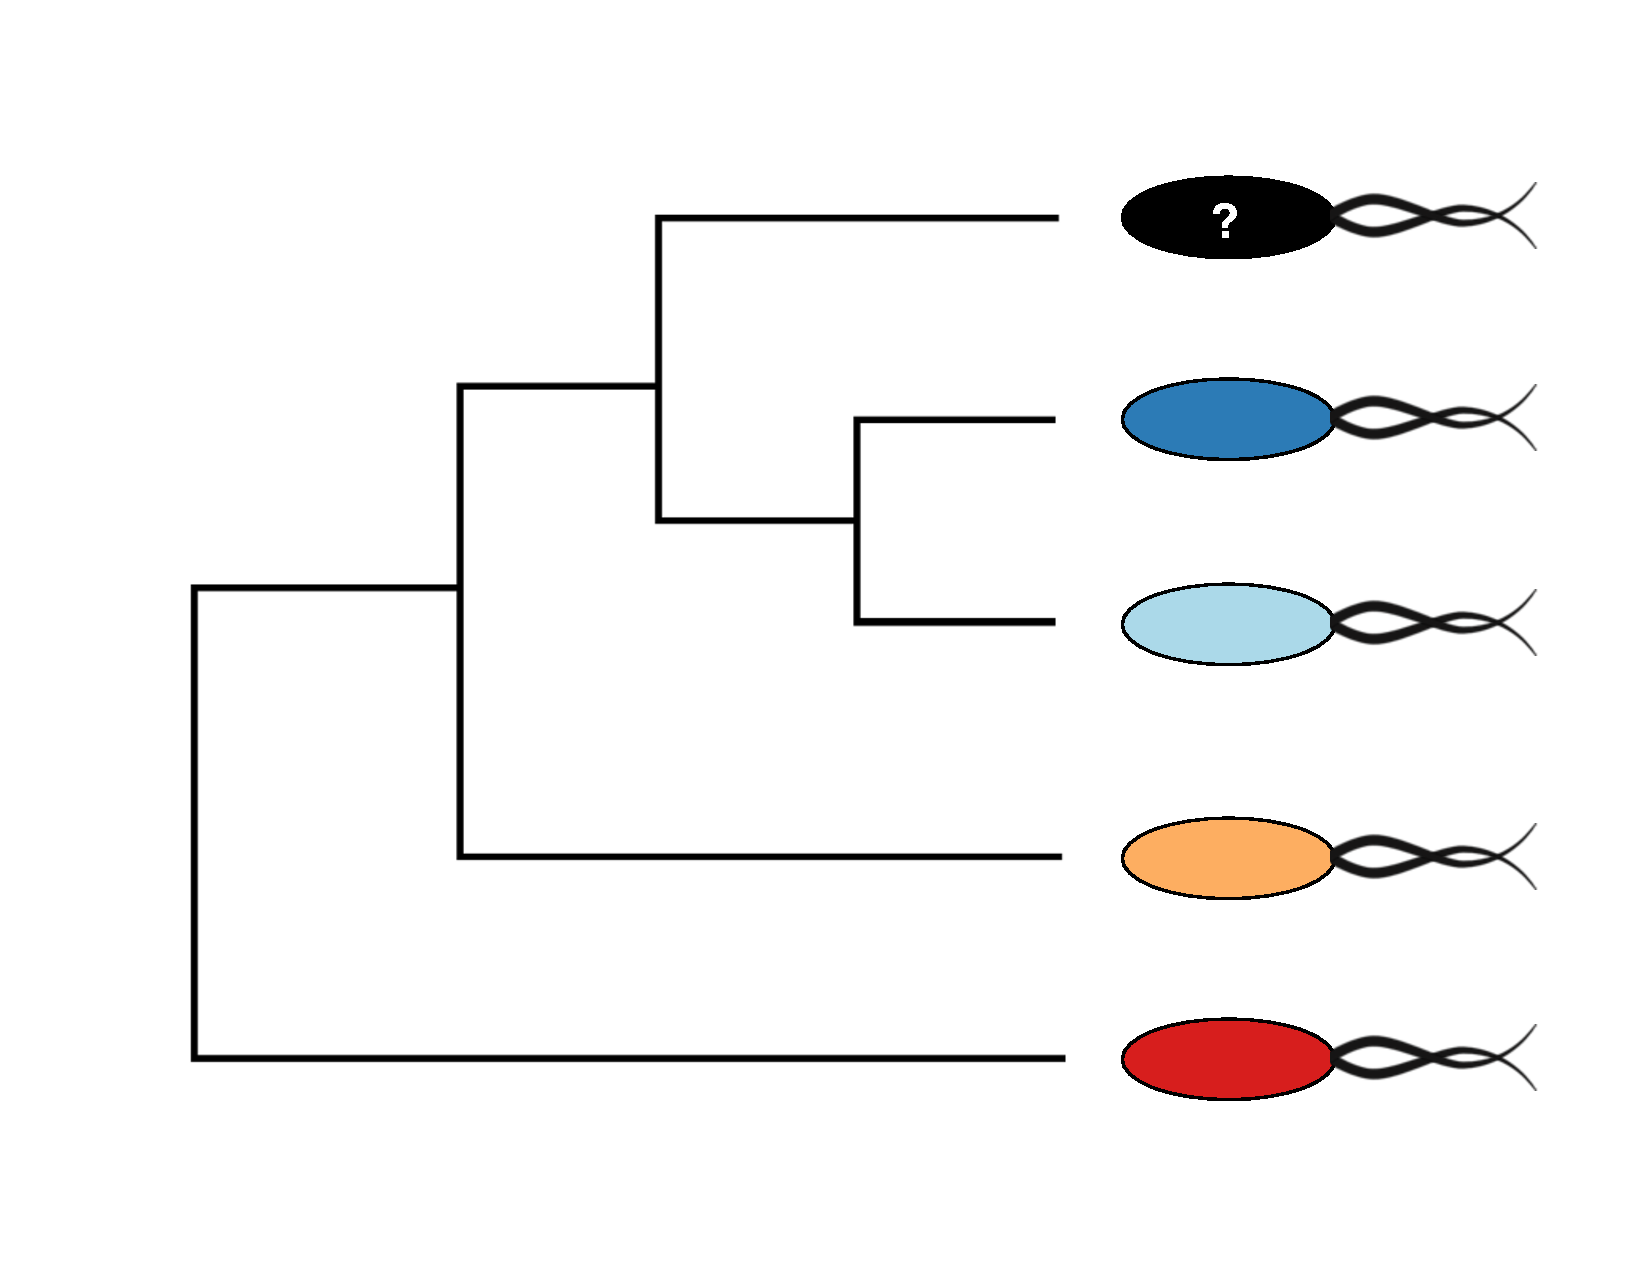
\includegraphics[width=0.6\textwidth]{media/compare-phylogenetically.pdf}
	 \caption{The pathways possessed by a novel organism (black) can be compared to those of closely related species to find out how this organism differs from its sister taxa.}
	 \label{fig:phylogenetic-comparison}
\end{figure}

\begin{figure}[!ht]
  \centering
	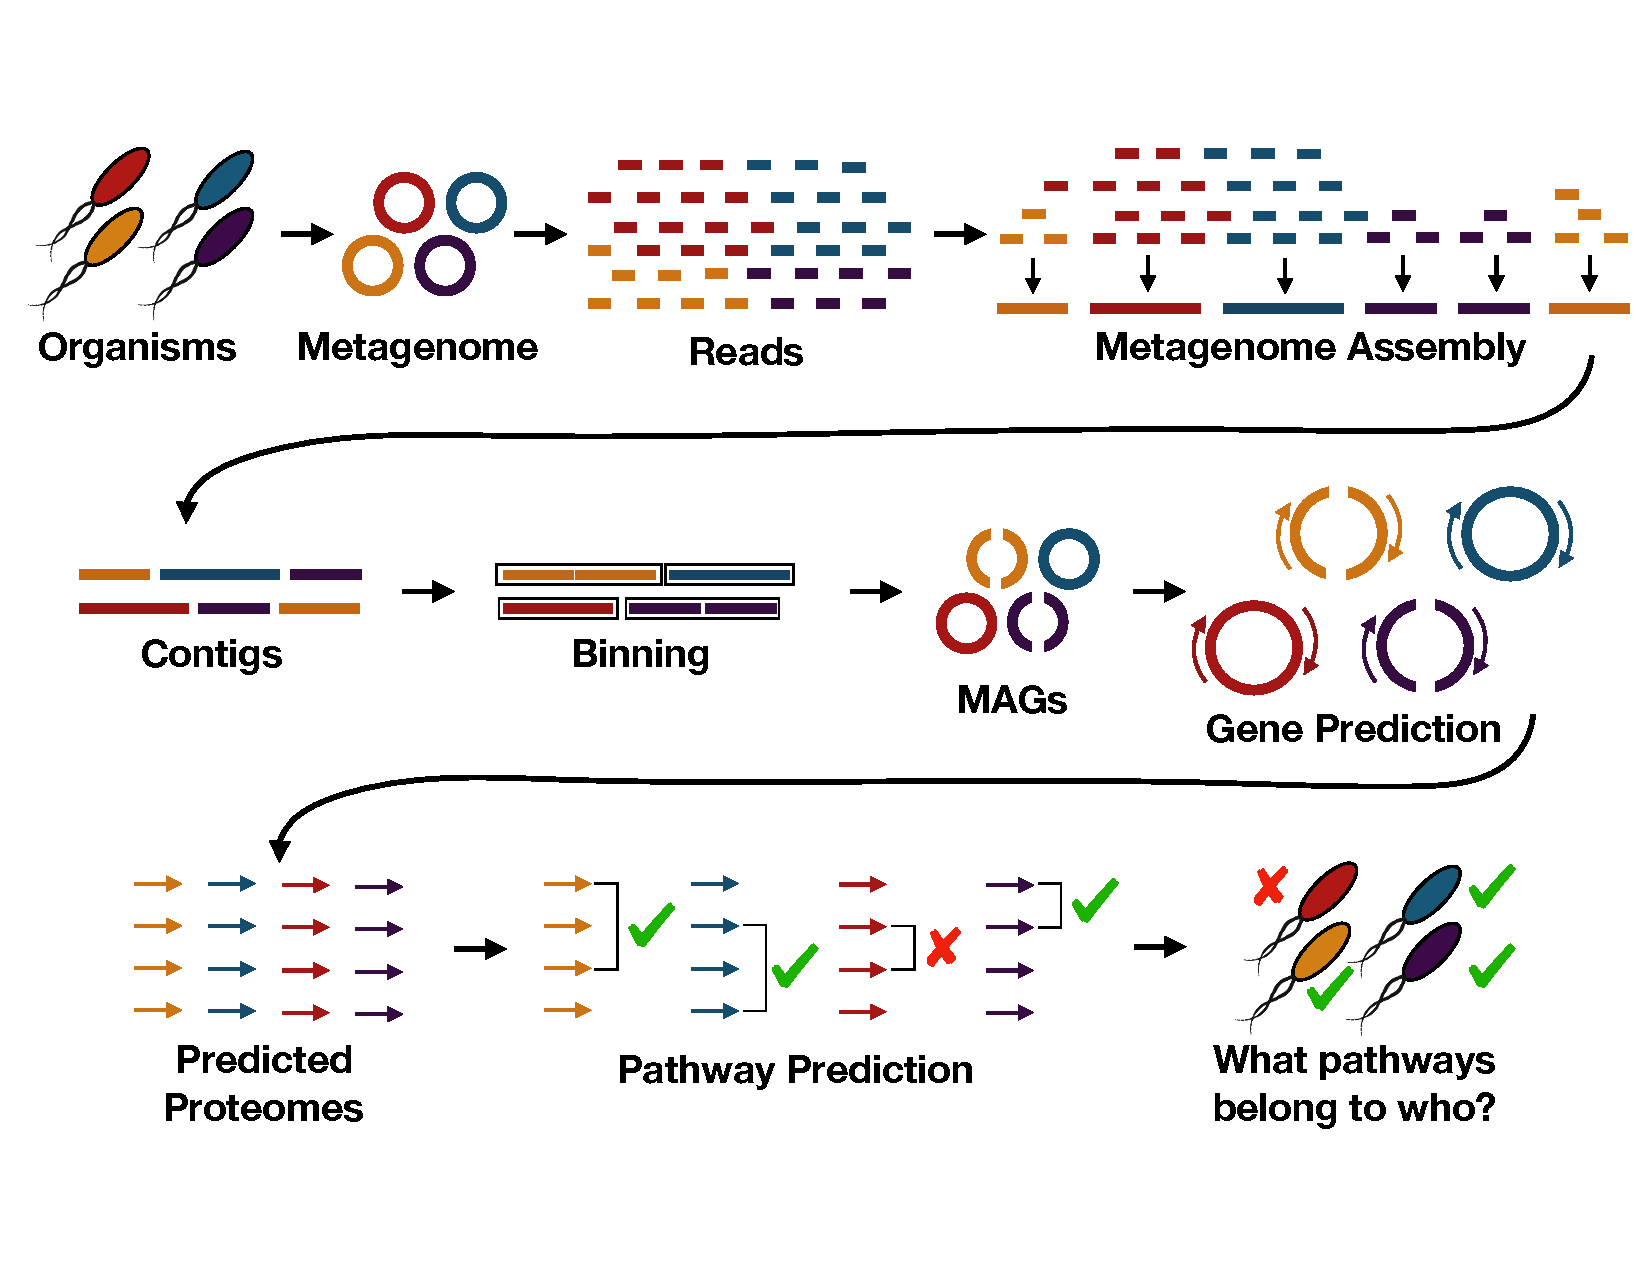
\includegraphics[width=0.8\textwidth]{media/metagenomics.pdf}
	 \caption{Metagenomics involves comparisons of multiple organism genomes found within the same environmental sample. As discussed in Footnote \ref{metagenomics-footnote}, bioinformatics techniques can be used to separate individual genomes from a metagenomic sample. Pathway annotation can be performed on these genomes and used to compare the pathways possessed by different organisms from the same environment. Such comparisons can be used to evaluate each organism's potential role in an environment.}
	 \label{fig:metagenomics}
\end{figure}

Although assigning pathway presence and absence to individual organisms can be done quite rapidly, the comparison of these results across multiple organisms is currently a considerable bottleneck in pathway analysis. Often pathway annotation tools that can process multiple genomes simultaneously present their results in the form of computer spreadsheets (e.g. Microsoft Excel or Comma Separated Value (CSV) files \cite{RFC4180}). Users are required to manually scan through the thousands of pathway rows and organism columns of these spreadsheets to find pathway differences between organisms. Researchers with data science and coding skills may be able to generate custom R or Python scripts that assist them in this task by filtering down these spreadsheets to show only pathways that are different or by generating data visualizations that accelerate pattern detection. To accelerate script development, libraries have been written to help scriptwriters interact with pathway data. However, the majority of these libraries focus on helping users download data from existing pathway databases, rather than helping them with making comparisons across organisms. Thus due to a lack of libraries for pathway comparison and lack of coding skills among biologists, there is a need for dedicated bioinformatics tools that enable the majority to easily and rapidly compare pathways across organisms. Software that visualizes the presence and absence of pathways across organisms would be of great use in this role. There are several emerging tools, which are discussed in Section \ref{micromeda-client-summary}, that help users visualize pathway annotations across organisms. However, their implementation, in terms of visual idioms used and supporting data presented, is currently lacking. There is currently a gap for a tool that effectively presents pathway annotation data and allows for rapid comparisons. There is also a gap for a pathway library that assists coders in making programmatic comparisons between the pathway annotations of multiple organisms. Also, there is a gap for a tool that can not only tell users what pathways an organism possess but also allows users to identify the protein sequences that support these annotations. Micromeda and Pygenprop were developed to fill these gaps.

\section{The Micromeda Platform}

The bioinformatics system presented within this thesis, called Micromeda, is designed to address current gaps in the researcher's ability to compare pathway presence and absence across organisms. The platform does so without losing information about the protein sequences that support these pathways' existence. The output of the platform is an interactive heat map consisting of rows of pathways by columns of organisms (Fig. \ref{fig:basic-heatmap-overview}). Heat map cells are coloured by the level of support for a pathway's existence in each genome (Fig. \ref{fig:basic-heatmap-overview}). This data visualization is displayed within a user's web browser. As discussed in Chapter \ref{micromeda-client}, this heat map is interactive, and users can customize it to only display presence and absence for specific pathways or pathway steps. A software stack (see \href{en.wikipedia.org/wiki/Solution\_stack}{en.wikipedia.org/wiki/Solution\_stack}) consisting of several components, some of which were developed as part of the thesis project, is used to generate data for the visualizations that Micromeda presents. This stack is outlined in the list below.

\begin{figure}[!ht]
  \centering
	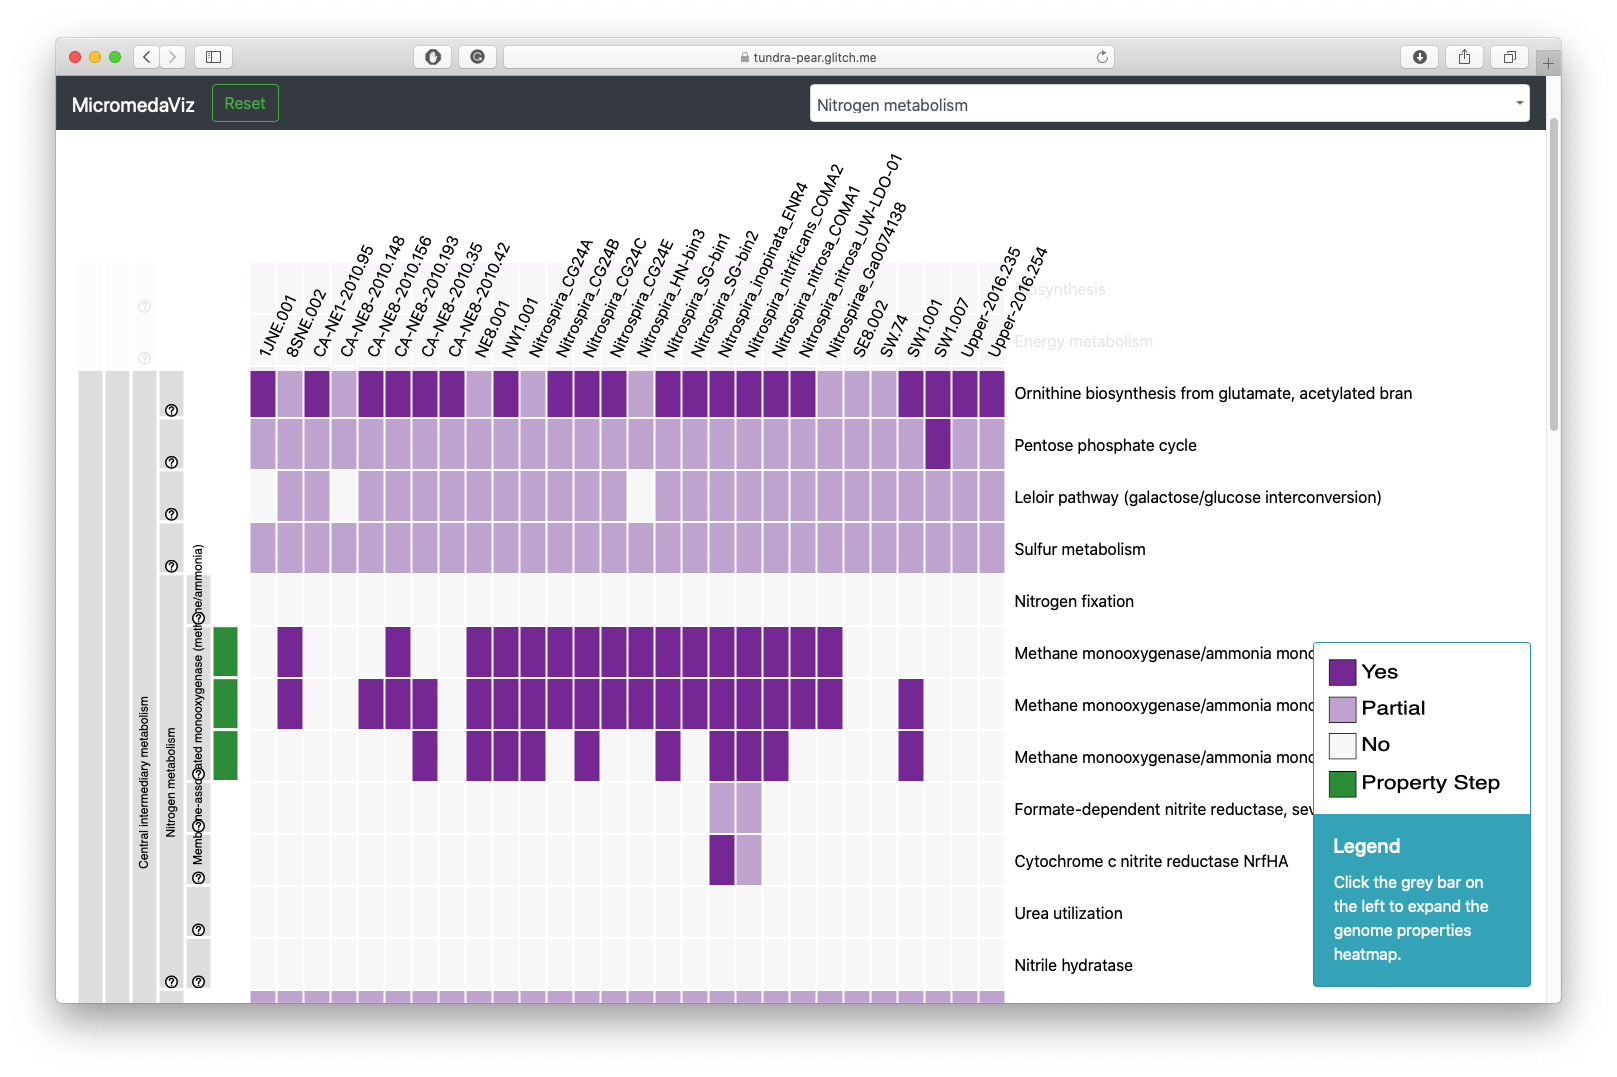
\includegraphics[width=0.8\textwidth]{media/Micromeda-Simple-Overview.png}
	 \caption{The genome properties database generates an interactive heat map of pathway rows by organism columns. A further explanation of the interface can be seen in Chapter \ref{micromeda-client}.}
	 \label{fig:basic-heatmap-overview}
\end{figure}

\begin{itemize}
\item A client web application that runs in the user's browser. This web application allows users to upload files to a server. These files contain precalculated data about an organism's predicted pathways and the protein sequences that support these predictions. This application draws the pathway heat maps mentioned above based on the data uploaded (Fig. \ref{fig:basic-heatmap-overview}). These heat maps allow users to make comparisons across pathways and organisms. This component is called \textbf{Micromeda-Client} and is detailed in Chapter \ref{micromeda-client}.
\item A server web application that runs on a remote computer system and in support of the client application. This server application accepts the above file upload and provides the client with easy access to the data held within the file. This component is called \textbf{Micromeda-Server} and is discussed in Chapter \ref{micromeda-server}.
\item A file format that allows users to easily transfer an assessment of what pathways are possessed by multiple organisms and the protein sequences used to support this assessment. These files, called \textbf{Micromeda files}, are the files uploaded to Micromeda-Server and use a custom format that is discussed in Section \ref{MicromedaFiles}. The format allows for the storage of the above information in the most compact way possible.
\item A software library that supports the generation of pathway annotations, rapid programmatic comparisons between organism pathway annotations and the generation of the above Micromeda files. The library is compatible with many emerging machine learning tools and opens up new avenues to their application to pathway analysis. This library is called \textbf{Pygenprop} and is discussed in Chapter \ref{Pygenprop}.
\item A pathway database that maps between predicted protein sequences derived from an organism's genome and biochemical pathway steps. The database chosen was the \textbf{Genome Properties} database \cite{richardson2018genome}. A short review of this database and the reason for its selection can be found in Chapter \ref{genome-properties}. This database is pre-existing and was not made as part of the thesis work.
\item A pre-existing sequence search program for scanning for identifying markers within the sequences of an organism's predicted proteins. These markers are used to identify enzymes that support the existence of a pathway. The search program chosen was \textbf{InterProScan5}, whose output data is used by the Genome Properties Database. An overview of InterProScan5 \cite{jones2014interproscan} and its methodology can be found in Chapter \ref{genome-properties}.
\item A program that generates protein sequences from predicted genes found within an organism's genome. For example, in the case of prokaryotic genomes, an existing tool such as \textbf{Prodigal} \cite{hyatt2010prodigal} would be used. 
\end{itemize}

\begin{figure}[!ht]
  \centering
	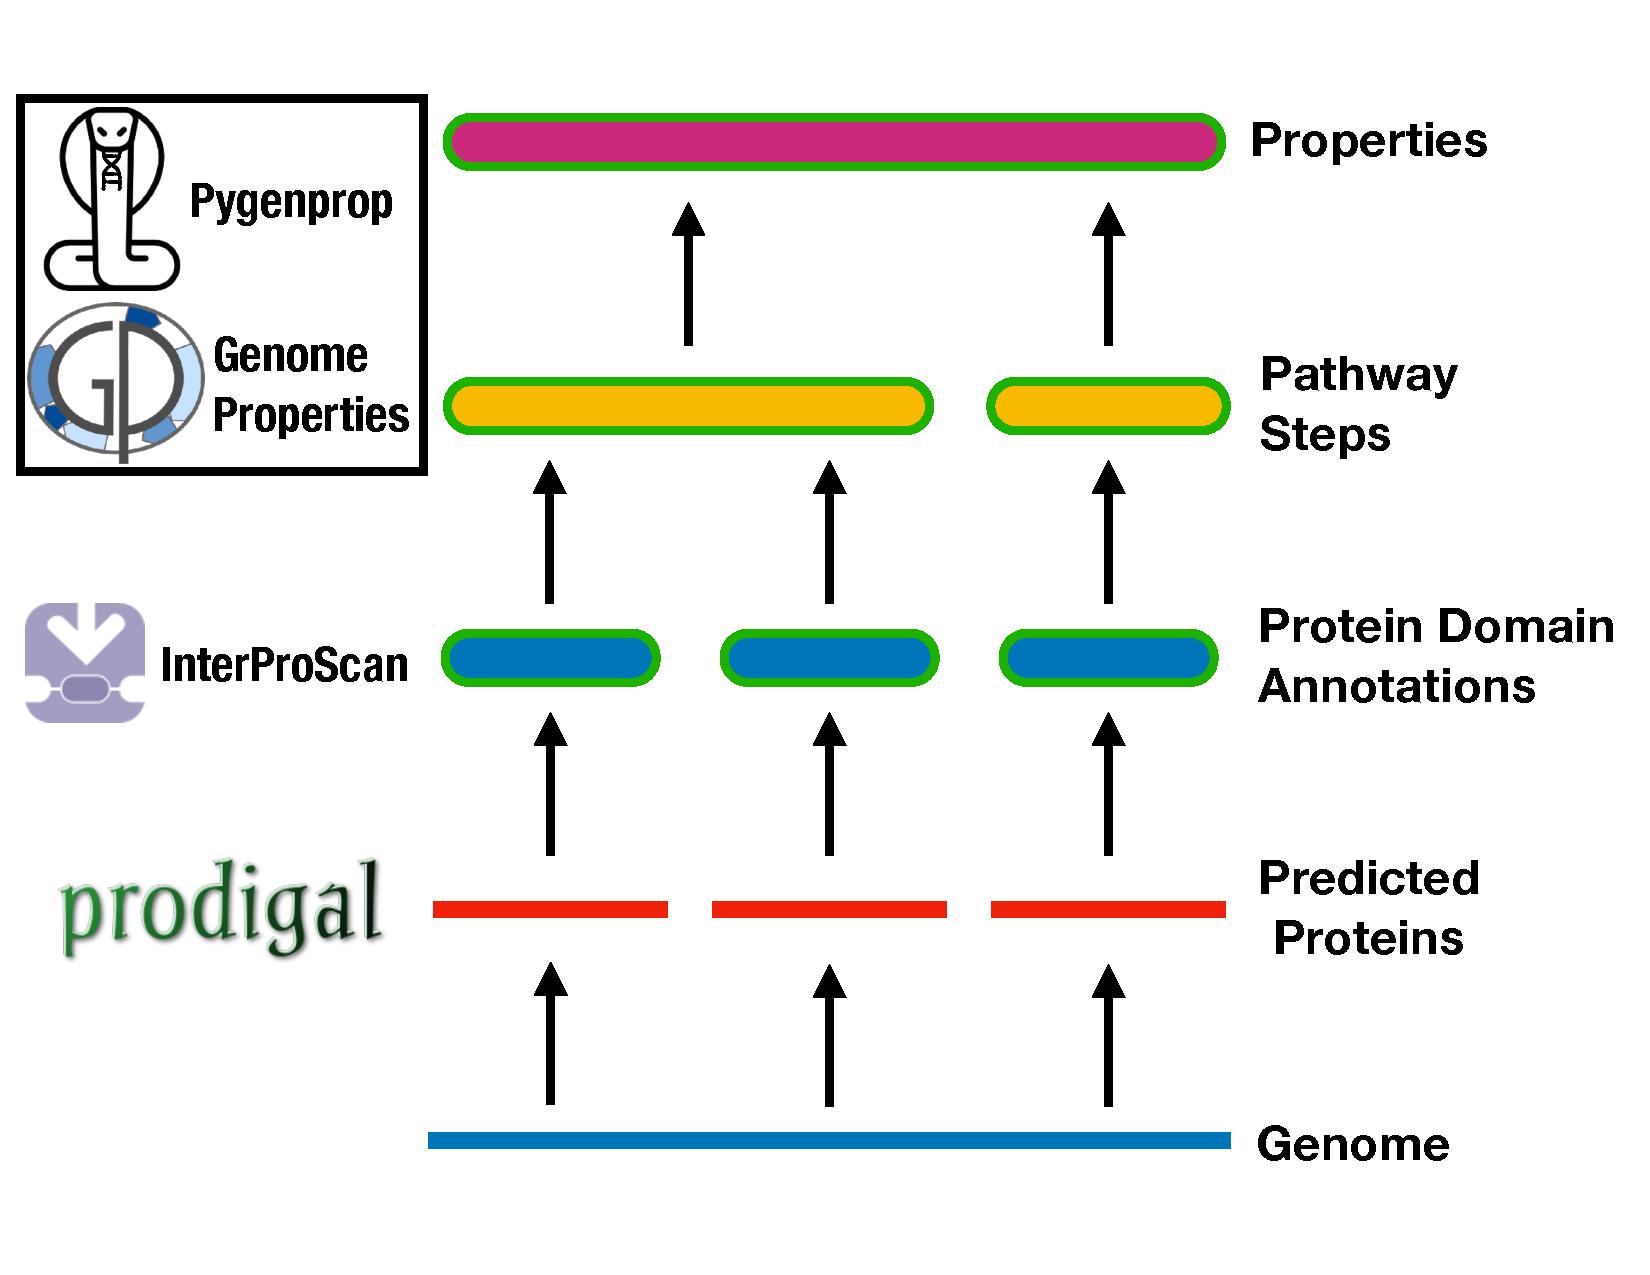
\includegraphics[width=0.8\textwidth]{media/micromeda-pipeline.pdf}
	 \caption{For prokaryotes, the process of generating pathway visualizations involves producing predicted proteins via Prodigal, scanning these proteins using InterProScan5 and then using the results to predict pathways using Pygenprop and a copy of the Genome Properties database.}
	 \label{fig:micromeda-levels}
\end{figure}

\begin{figure}[!ht]
  \centering
	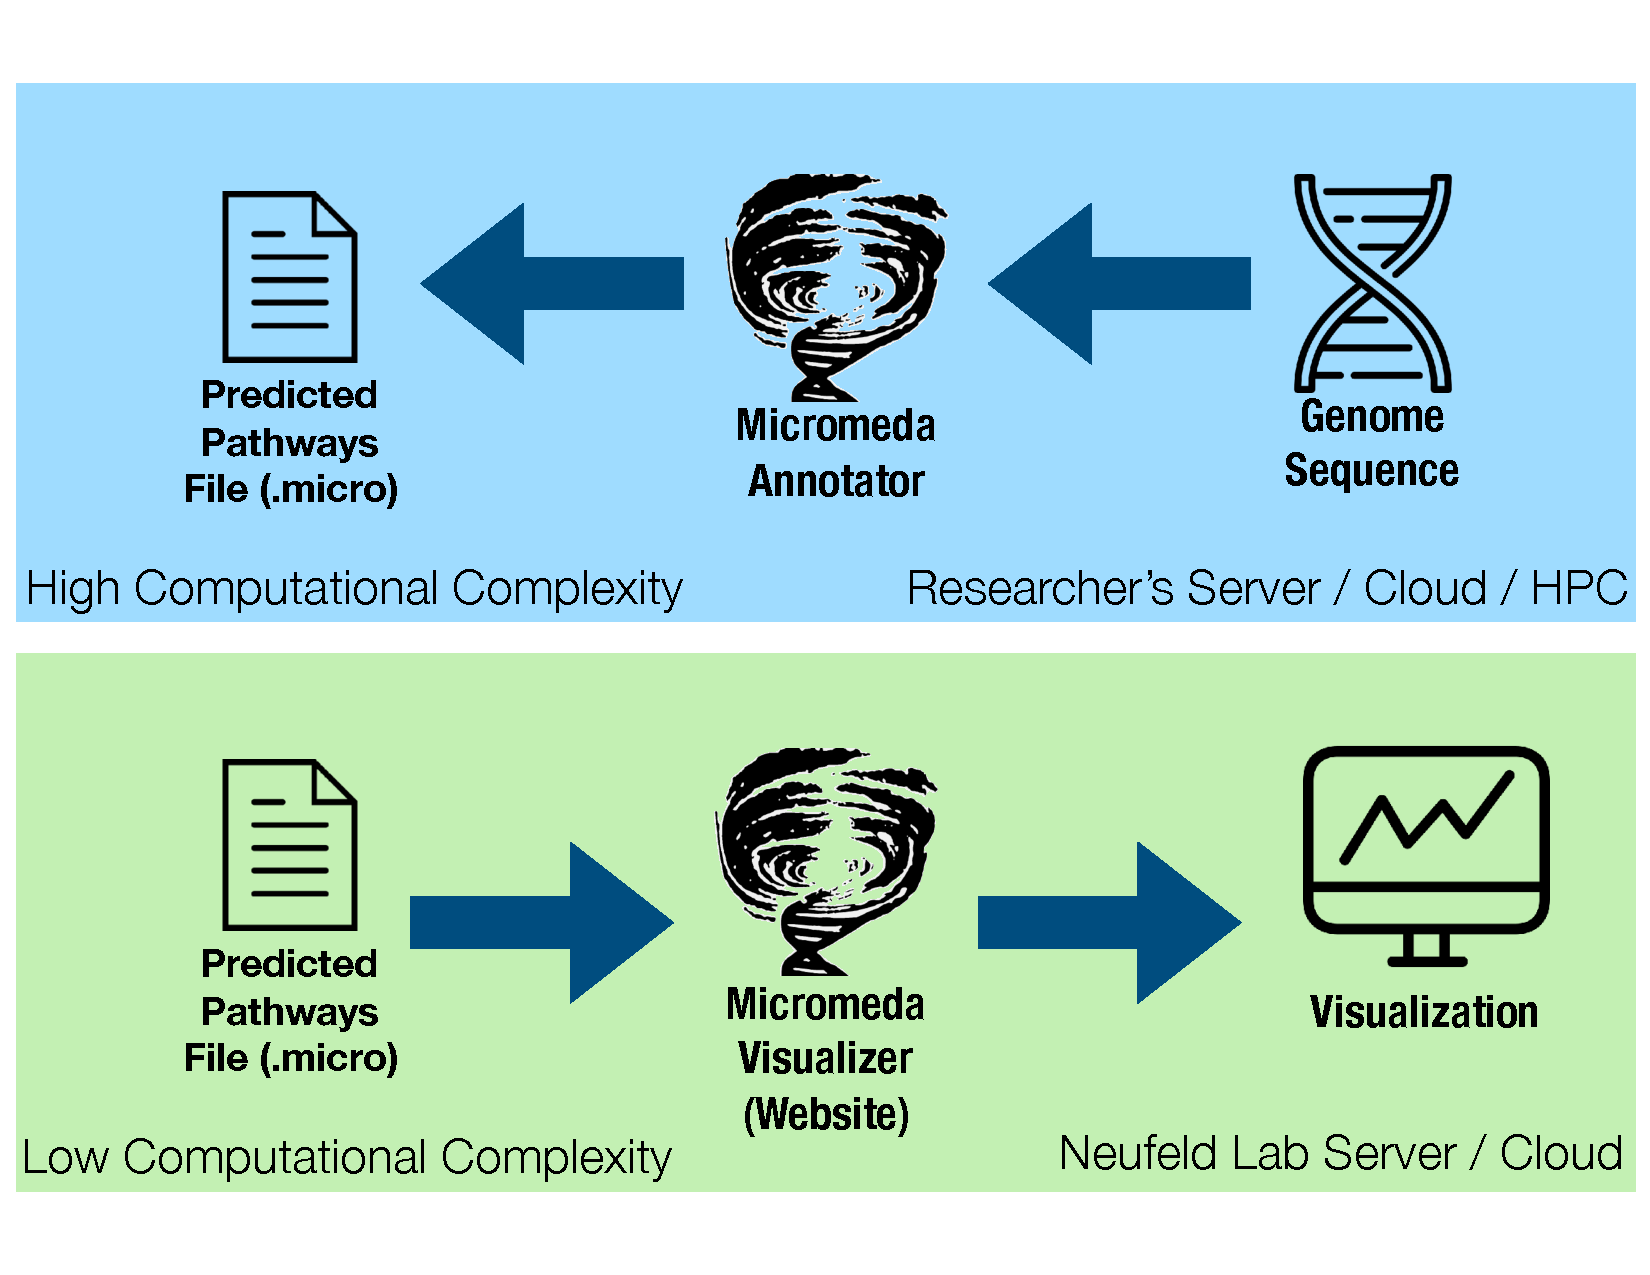
\includegraphics[width=\textwidth]{media/micromeda-file-generation.pdf}
	 \caption{Micromeda splits its computation into two components: a data generation step that creates Micromeda files and a visualisation step that involves the upload of this file to a remote server. The most computationally complex steps are not performed on the same computer as the visualisation.}
	 \label{fig:micromeda-file-generation}
\end{figure}

\begin{figure}[!ht]
  \centering
	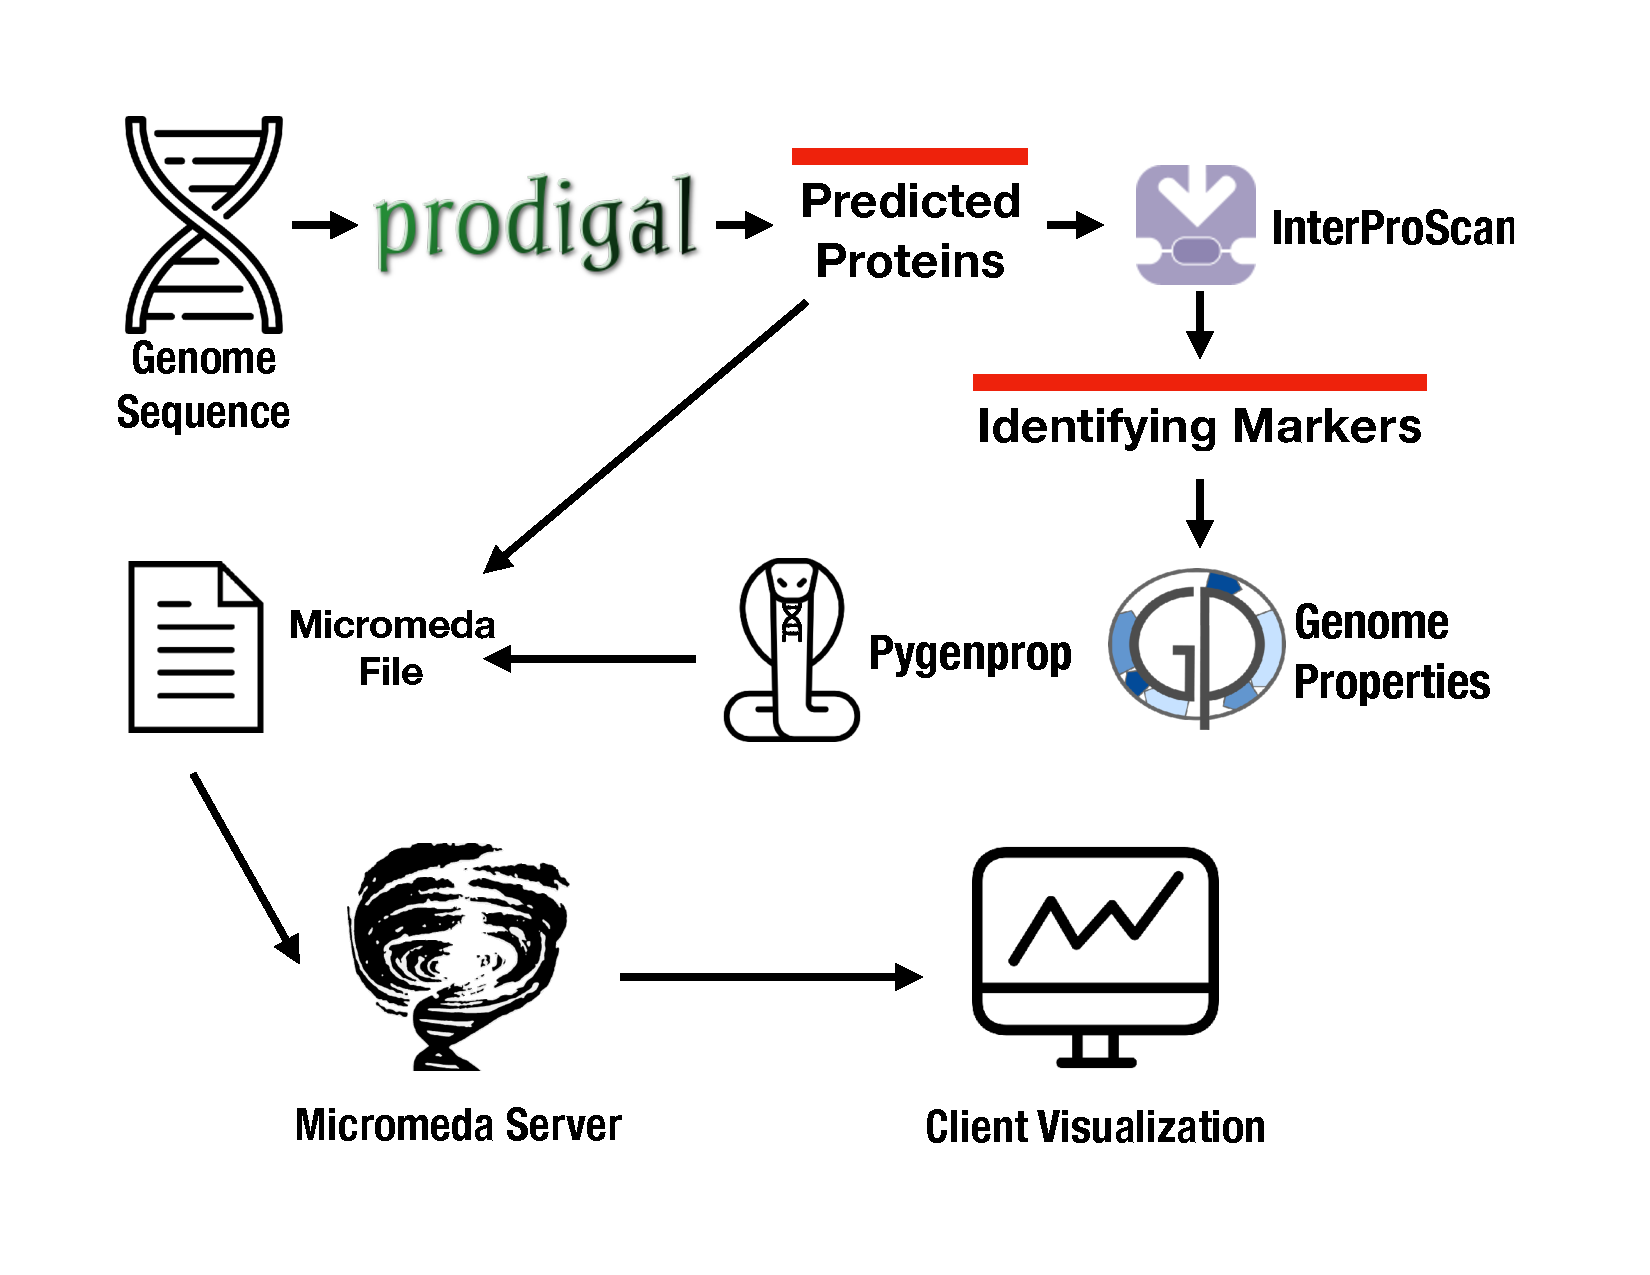
\includegraphics[width=0.8\textwidth]{media/how-micromeda-files-are-built.pdf}
	 \caption{Micromeda files are ultimately derived from InterProScan annotations of an organism's predicted proteins. The files contain both pathway annotations derived from these InterProScan proteins annotations as well as protein sequences. These files are uploaded to a remote server for visualization.}
	 \label{fig:micromeda-file-building-and-use}
\end{figure}

The above Micromeda platform can be subdivided into two core components: a toolchain for generating Micromeda files (labelled Micromeda Annotator in Fig. \ref{fig:micromeda-file-generation}) and a web application for visualizing the data they contain (labelled Micromeda Visualizer in Fig. \ref{fig:micromeda-file-generation}). The individual steps for generating Micromeda files can be done manually using only three command-line tools (Fig. \ref{fig:micromeda-levels} and Fig. \ref{fig:micromeda-file-building-and-use}). For example, with prokaryotic genomes, Prodigal could be used to predict protein sequences from an organism's genome sequence, and InterProScan5 could be used to scan these proteins to identify enzymes that support the existence of specific pathways (Fig. \ref{fig:micromeda-file-building-and-use}). Afterwards, a Python script that uses the Pygenprop library could be used to convert the output from InterProScan and Prodigal into Micromeda files. This script would use both Pygenprop and a copy of the Genome Properties database (Fig. \ref{fig:micromeda-file-building-and-use}). An example of such a script can be found within Pygenprop's Github repository. An explicit automated software pipeline for generating Micromeda files does not currently exist. However, its potential implementation is discussed in Section XXX.

\subsection{Software Architecture Overview}

Micromeda follows a client-server web architecture \cite{svobodova1985client} (see \href{en.wikipedia.org/wiki/Client–server\_model}{en.wikipedia.org/wiki/Client –server \_model} and Section \ref{web-servers}). Users interact with Micromeda-Client via their web browser, and it allows them to upload Micromeda files to Micromeda-Server. The Micromeda files contain all the information that the client requires to generate a pathway heat map. These files store pathway annotations, InterProScan5 output data, and supporting protein sequences for multiple organisms (see Section \ref{MicromedaFiles}). Having all these datasets in a single file simplifies the data upload process as only one file has to be uploaded by the user per heat map drawn rather than multiple. After upload, the contents of the uploaded file are stored temporarily in Random Access Memory (RAM) on the computer used to host Micromeda-Server (see Section \ref{server-workflow}). Micromeda-Client will ask Micromeda-Server for data from this file as it draws a heat map or responds to user activity (see Section \ref{client-implementation}). Multiple users can interact with Micromeda-Server and Client simultaneously.

\subsection{The reasoning for building a Web Application and having Micromeda files} \label{why-micromeda-files}

The reasons for choosing a web-based architecture for Micromeda versus building it as a client desktop application are discussed in Section \ref{client-delivery-method}. There are vast computational complexity differences between creating Micromeda files and visualizing their contents. Micromeda's pathway prediction method involves identifying specific enzymes by running InterProScan5 on the set of all predicted proteins of an organism. The algorithms used by InterProScan5 are very computationally complex. It takes on the order of two hours to scan through the 4313 proteins of E. coli K12 using 100\% of all the Central Processing Unit (CPU) cores of a 16 core server \footnote{InterProScan5 was tested on a server with two Intel E5310 (4 core/4 threads/8M cache/1.60GHz clock) processors and 16GB of Random Access Memory (RAM).}. In contrast, Micromeda can render a pathway heat map for over twenty organisms in only a few seconds. There are six orders of magnitude difference in terms of wall time (see \href{en.wikipedia.org/wiki/Elapsed\_real\_time}{en.wikipedia.org/wiki/Elapsed\_real\_time}), between gathering the data for a heat map and rendering it. Thus, if one wanted to have a web application that both computes and visualizes pathway annotations for uploaded genome sequences, it would require the support of an extensive and well-maintained hardware infrastructure. Such an infrastructure would require at least one dedicated web server with many CPU cores or even a compute cluster. This system's main focus would be to run InterProScan5 rather than generate heat maps for users. Such as system would require a job scheduler implemented to maintain fair use and prevent overload \footnote{A job scheduling system would help ensure that upon the upload of a large number of genomes, they would be processed in batches to prevent a processing server from being overwhelmed. A scheduler would also be vital for allowing multiple users to annotate pathways fairly. Should a user who just uploaded one hundred genomes have a preference, in terms of results turn around time, over a user who just uploaded a single genome a few seconds later? Selecting a scheduling system that is not first-come, first-served (FCFS) would allow the second user to get their results sooner.}. Developing the code to build, maintain and sustain such a system draws away from the core goal of the Micromeda platform, which was to build a tool that helps users visualize pathway differences across organisms. Thus, for Micromeda, it was chosen to have users generate their own Micromeda files, using InterProScan5 and other tools, on their computers (or temporary cloud computers) and have them upload these files to a remote web server for visualization (Fig. \ref{fig:micromeda-file-generation}). This design decision significantly reduces the hardware requirements for those who want to host Micromeda-Server and Client. It also reduces the overall design complexity of Micromeda-Client and Server and allows future development to focus on creating better and more feature-rich versions of Micromeda's user interface and visualization.


\section{Summary}

Micromeda allows users to visualize the differences in pathway presence and absence across organisms. It does this based on the data contained within uploaded Micromeda files. Pygenprop is a software library that can not only produce Micromeda files but also make programmatic comparisons of pathway presence and absence across organisms. Potential improvements to individual components of Micromeda are highlighted in the summary section of each of their chapters. Potential improvements that would require modification of multiple components are highlighted in Chapter XXX. As discussed in Chapter XXX, Micromeda breaks new ground in both features and implementation and will increase both the speed and ease at which researchers perform pathway analysis.
